\documentclass[11pt,a4paper]{article}
\usepackage{graphicx}
\usepackage{amssymb}
\usepackage{float}
\DeclareGraphicsExtensions{.pdf,.png,.jpg}

\begin{document}

\title{CS6690: Pattern Recognition Assignment \#2}
\author{Group 3: Akshay \& Suthirth}
\maketitle

\newpage

\section{Bayesian Classifiers}
According to Bayes Theorem, for a dataset x with classes $\omega_i$, \\
Probability of a datapoint belonging to class $\omega_i$ is defined as: \\
\begin{equation}
P(\omega_i | x) = \frac{(P(x|\omega_i)P((\omega_i))}{P(x)}
\end{equation}
\\ 

\begin{itemize}

	\item Here, $P(x|\omega_i)$ is known as the class likelihood. 
\\ To estimate this value, we require the distribution of $\omega_i$.
Based on the central limit theorem, we can assume that this would be Gaussian distribution for large datasets. 

	\item The value $P(\omega_i)$ is the class prior and is calculated using:
		\begin{equation}
		P(\omega_i) = N_i / N  
		\end{equation}
	This term becomes irrelevant if the classes have equal probabilities. 

	\item P(x) is termed as 'evidence' and can be calculated as:
	\begin{equation}
	{P(x) = \sum_i P(x | \omega_i)P(\omega_i)}
	\end{equation}
\end{itemize}

\section{Gaussian Likelihood Distribution}
 
 For multi-dimensional data, the Gaussian Distribution is:   
 \begin{equation}
 P(x;\mu,\Sigma) = \frac{1}{2\pi^{k/2}|\Sigma|^{1/2}} e^{-(x-\mu)^{T} \Sigma^{-1} (x-\mu)}
 \end{equation}
 
 where
 \begin{itemize}
 	\item $\mu$ is the mean 
 	\item $\Sigma$ is the covariance matrix
 \end{itemize}
 
 The above parameters are calculated for the following cases:
 \subsection{Bayes Classifier with Covariance same for all classes}
 \subsection{Bayes Classifier with Covariance different for all classes}
 \subsection{Naive Bayes Classifier with C = $\Sigma^2*I$}
 \subsection{Naive Bayes Classifier with C same for all classes}
 \subsection{Naive Bayes Classifier with C different for all classes} 

\section{Bayes Classification}

If $P(\omega_1 | x) > P(\omega_2 | x)$ then x belongs to class $\omega_1$
\\If $P(\omega_1 | x) < P(\omega_2 | x)$ then x belongs to class $\omega_2$\\

Using equation (1), this can be written as:
 \begin{equation}
 {P(x| \omega_1)P(\omega_1) \gtrless P(x | \omega_2)P(\omega_2)}
 \end{equation}

This classification rules minimizes number of misclassifications. 

\clearpage
\section{Experiments}

\subsection{Data}
Red - Class 1, Green - Class 2, Blue - Class 3, Cyan - Class 4\\
Black (solid) - 1st Eigenvector\\
Black (dashed) - 2nd Eigenvector\\  
\begin{figure}[H]
		\centering
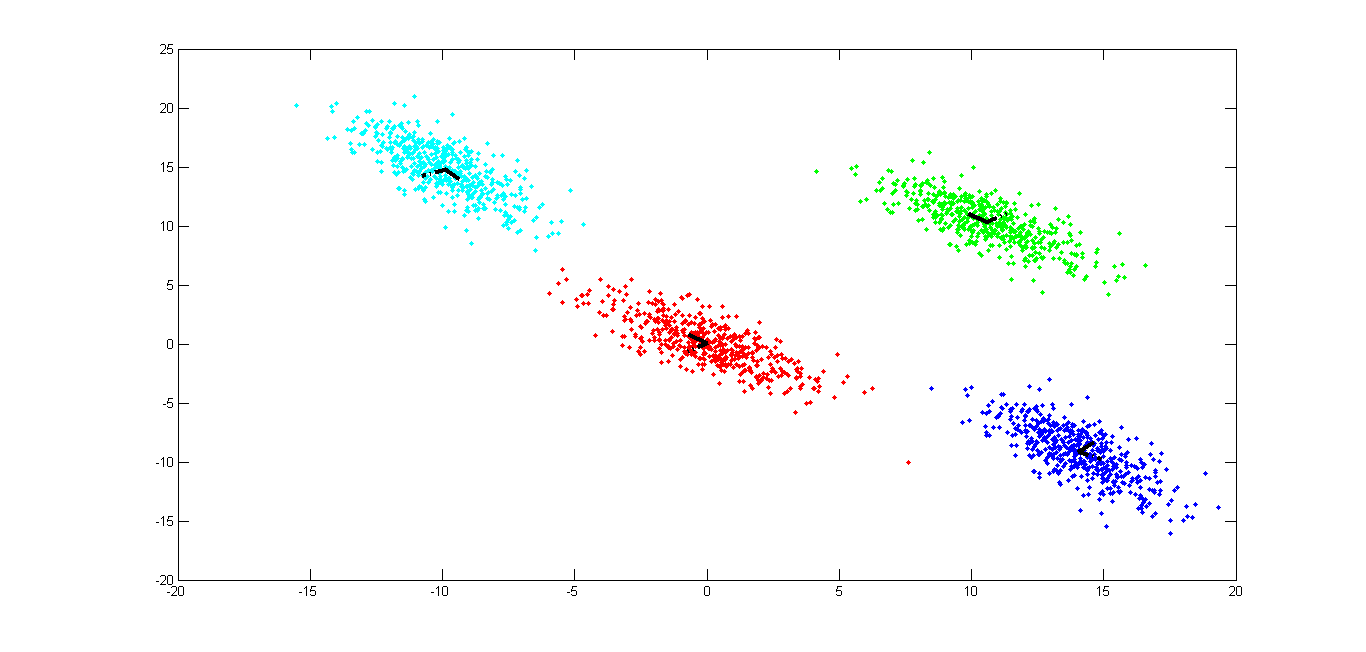
\includegraphics[height=7cm]{Figures/ls_eig.png}
\caption{Linearly Separable Data}
\end{figure}

\begin{figure}[H]
		\centering
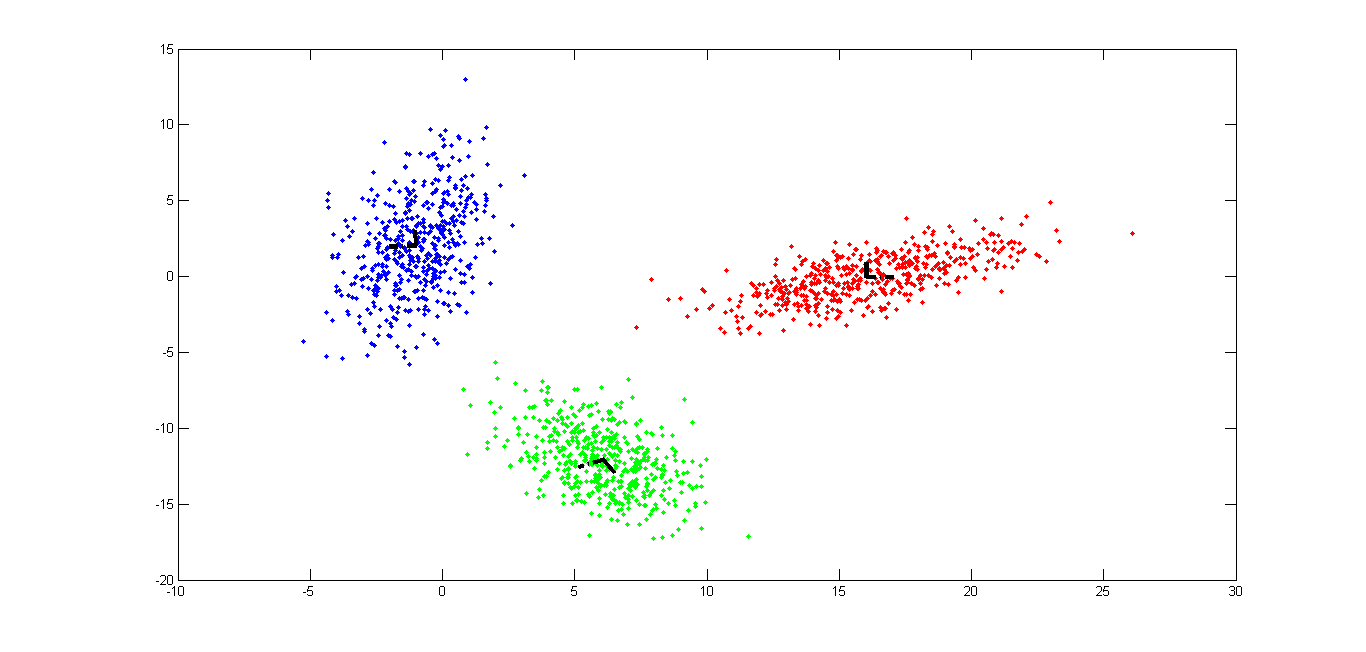
\includegraphics[height=7cm]{Figures/NLS_eig.png}
\caption{Non-linearly Separable Data}
\end{figure}

\clearpage
\begin{figure}[H]
		\centering
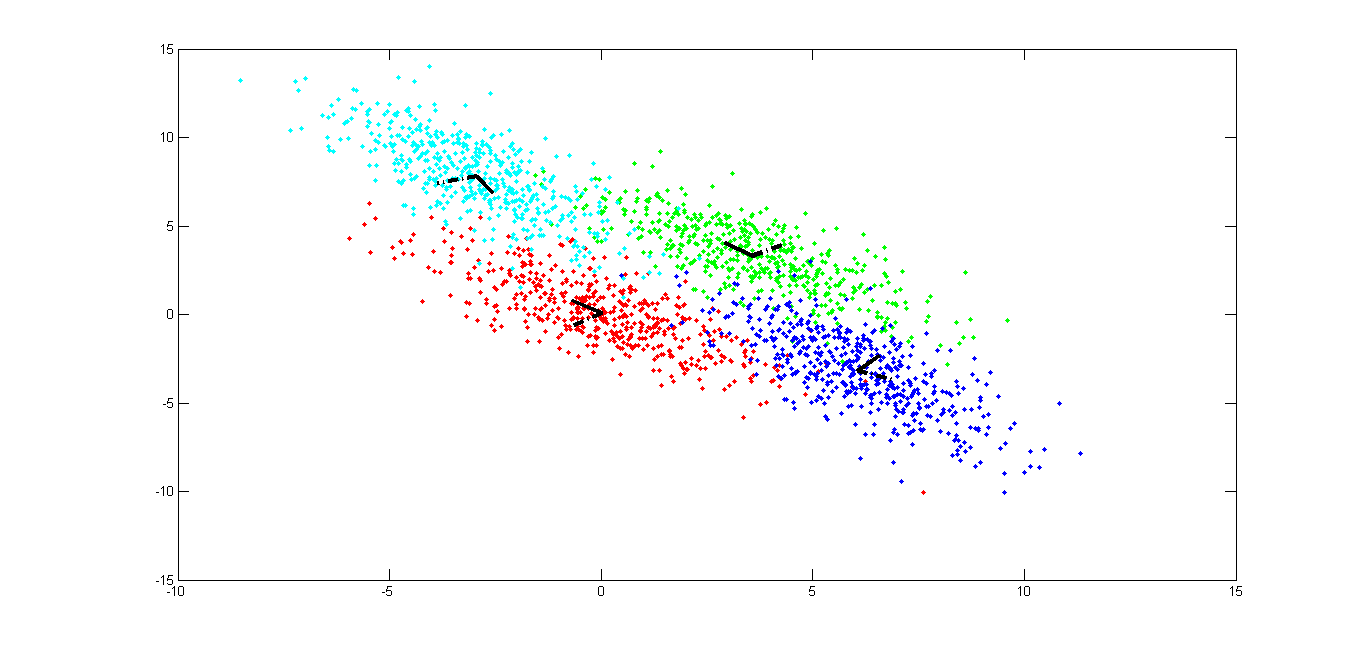
\includegraphics[height=7cm]{Figures/OD_eig.png}
\caption{Overlapping Data}
\end{figure}

\begin{figure}[H]
	\centering
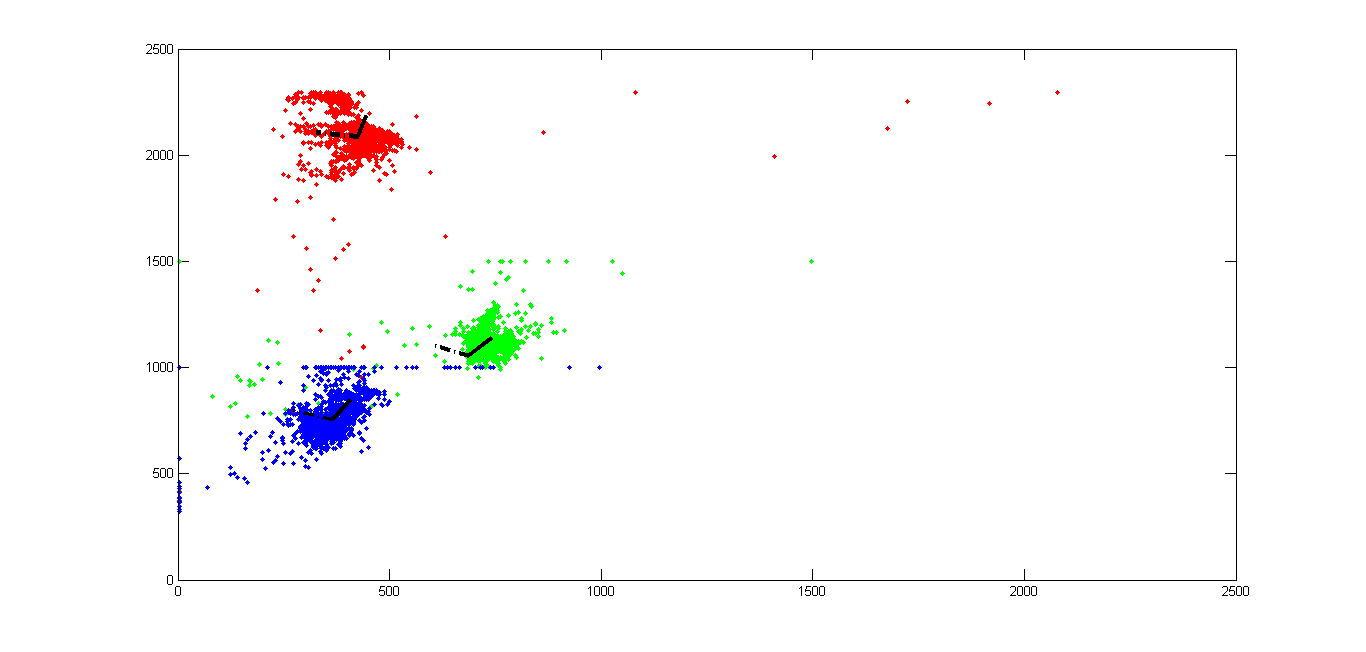
\includegraphics[height=7cm]{Figures/RWD_eig.png}
\caption{Real World Data: Vowel utterance formant frequencies F1 and F2}
\end{figure}

\clearpage
\subsection{Decision Boundaries}
Following plots describe the decision boundaries for various datasets with different Bayesian classifiers. \\

For every figure,\\
\textbf{Row 1:} Bayes with: (L) Same covariance for all classes, (R) Different covariance for all classes\\
\textbf{Row 2:\textbf{}} Naive Bayes with: (L) $C = \Sigma^2*I$, (R) Same C for all classes\\
\textbf{Row 3:} Naive Bayes with different C for all classes\\

\underline{\textbf{Legends:}}\\
Red - Class 1\\
Green - Class 2\\
Blue - Class 3\\
Cyan - Class 4\\
White - $\mu_1 - \mu_2, \mu_3, \mu_4$\\
Yellow - Decision Boundary b/w Class 1 and 2 \\
Magenta - Decision Boundary b/w Class 1 and 3 \\
Cyan (line) - Decision Boundary b/2 Class 1 and 4 

\begin{figure}[H]
	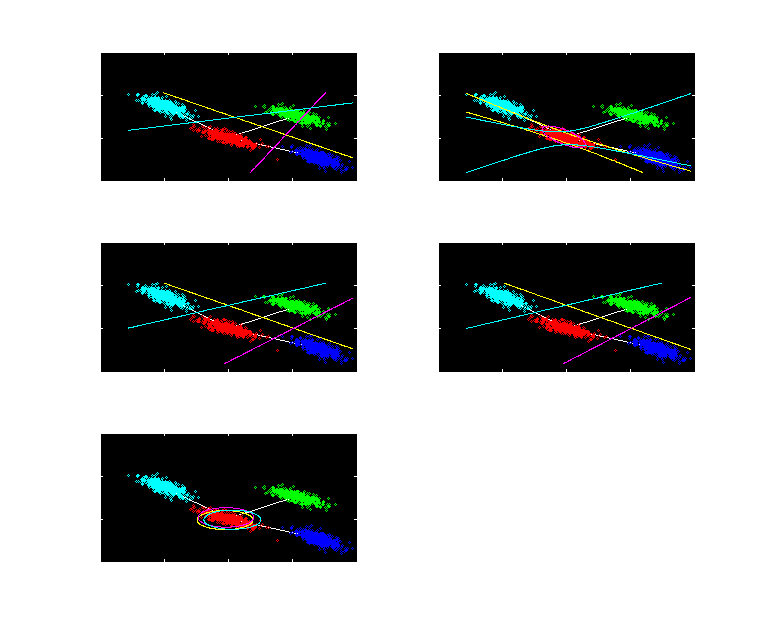
\includegraphics[height=9cm]{Figures/LS_DB.png}
	\caption{Linearly Separable Data}
\end{figure}

\begin{figure}[H]
	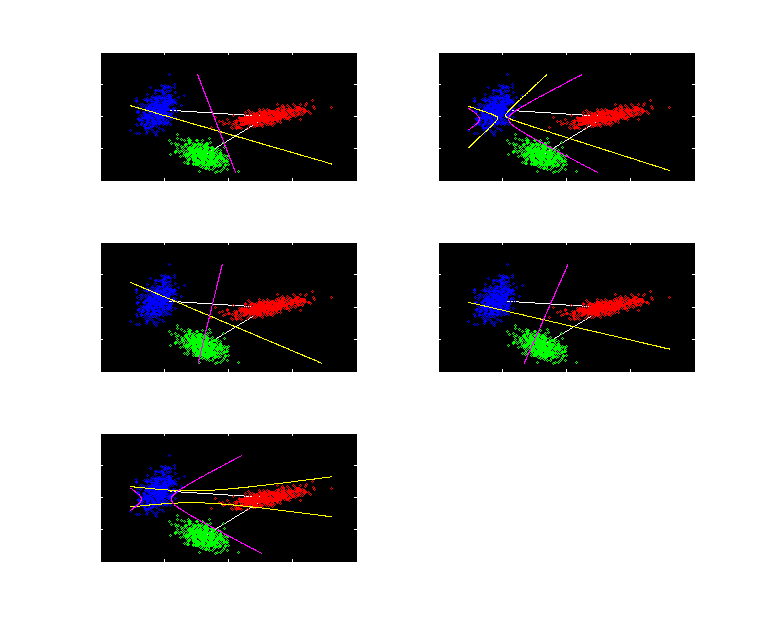
\includegraphics[height=9cm]{Figures/NLS_DB.png}
	\caption{Non-linearly Separable Data}
\end{figure}

\begin{figure}[H]
	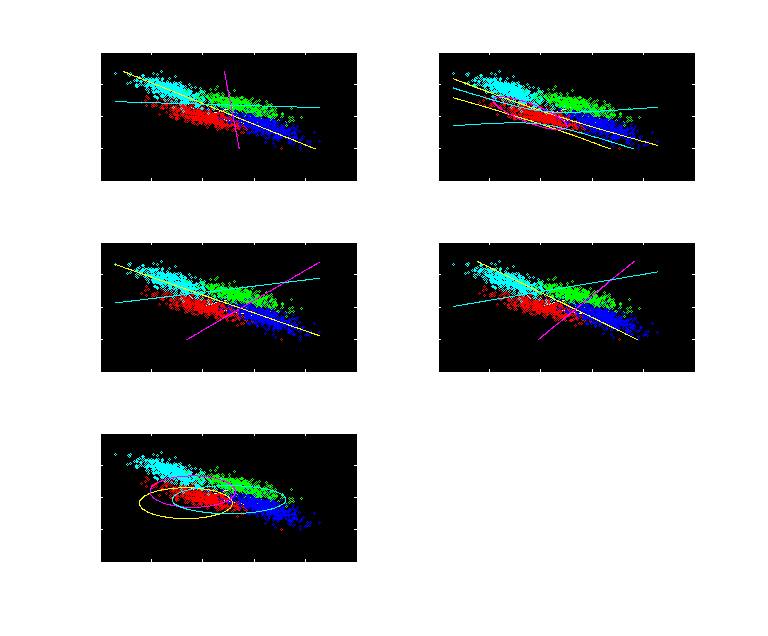
\includegraphics[height=9cm]{Figures/OD_DB.png}
	\caption{Overlapping Data}
\end{figure}

\begin{figure}[H]
	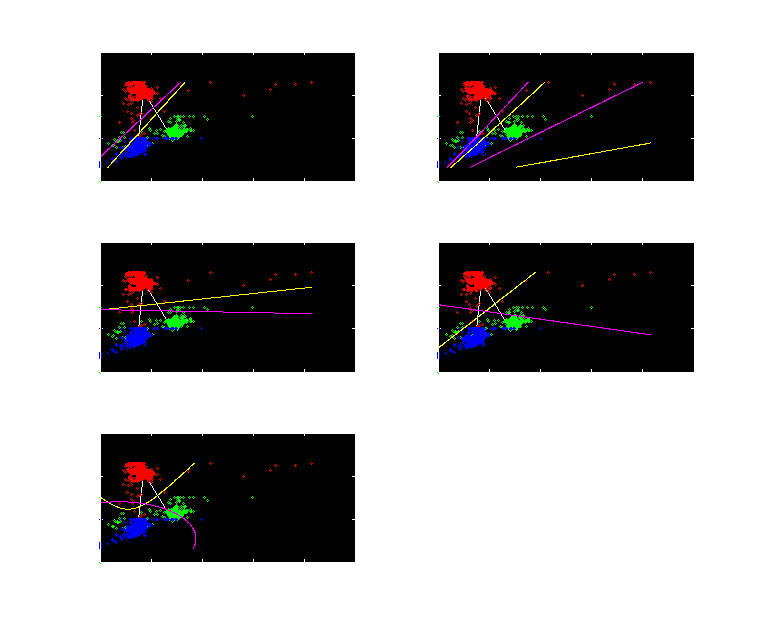
\includegraphics[height=9cm]{Figures/RWD_DB.png}
	\caption{Real World Data: Formant frequencies F1 and F2 for vowel utterances}
\end{figure}


\subsection{Confusion Matrices}

\section{Cases}

\section{Conclusion}
Write your conclusion here.

\end{document}